\documentclass[10pt,aspectratio=169]{beamer}
% \documentclass[10pt,aspectratio=169,handout]{beamer}

% silence some Metropolis warnings
\usepackage{silence}
\WarningFilter{beamerthememetropolis}{You need to compile with XeLaTeX or LuaLaTeX}
\WarningFilter{latexfont}{Font shape}
\WarningFilter{latexfont}{Some font}

% define custom colors
\definecolor{dark gray}{HTML}{444444}
\definecolor{light gray}{HTML}{777777}
\definecolor{dark red}{HTML}{BB0000}
\definecolor{dark green}{HTML}{00BB00}

% configure metropolis
\usetheme[numbering=fraction]{metropolis}
\setbeamercolor{background canvas}{bg=white}
\setbeamercolor{frametitle}{bg=dark gray}
\setbeamercolor{alerted text}{fg=dark red}
\setbeamercolor{item projected}{bg=dark red}
\setbeamercolor{local structure}{fg=dark red}
\setbeamersize{text margin left=0.5cm,text margin right=0.5cm}
\setbeamercovered{transparent=10}

% use thicker lines
\makeatletter
\setlength{\metropolis@titleseparator@linewidth}{1pt}
\setlength{\metropolis@progressonsectionpage@linewidth}{1pt}
\makeatother

% custom bullet points
\setbeamertemplate{itemize item}{\color{dark red}$\blacktriangleright$}
\setbeamertemplate{itemize subitem}{\color{dark red}$\blacktriangleright$}
\setbeamertemplate{itemize subsubitem}{\color{dark red}$\blacktriangleright$}
\newcommand{\custombullet}{{\color{dark red}$\blacktriangleright$}\hspace{0.5em}}

% use classic font for math
\usefonttheme[onlymath]{serif}

% imports
\usepackage[english]{babel}
\usepackage[utf8]{inputenc}
\usepackage{amsthm}
\usepackage{amssymb}
\usepackage{amsmath}
\usepackage{amsfonts}
\usepackage{mathtools}
\usepackage{mathabx}
\usepackage{stmaryrd}
\usepackage{graphicx}
\usepackage{hyperref}
\usepackage{xfrac}
\usepackage{appendixnumberbeamer}

% check and x marks
\usepackage{pifont}
\newcommand{\cmark}{{\color{dark green}\ding{51}}\hspace{0.3em}}
\newcommand{\xmark}{{\color{dark red}\ding{55}}\hspace{0.5em}}

% diagrams
\usepackage{tikz}
\usetikzlibrary{decorations.pathreplacing}

% references
\usepackage[natbibapa]{apacite}
\bibliographystyle{apacite}
\renewcommand{\bibsection}{}

% use ampersands instead of "and" for text citations
\AtBeginDocument{\renewcommand{\BBAB}{\&}}

% possessive cites
\makeatletter
\patchcmd{\NAT@test}{\else \NAT@nm}{\else \NAT@nmfmt{\NAT@nm}}{}{}
\DeclareRobustCommand\citepos
  {\begingroup
   \let\NAT@nmfmt\NAT@posfmt
   \NAT@swafalse\let\NAT@ctype\z@\NAT@partrue
   \@ifstar{\NAT@fulltrue\NAT@citetp}{\NAT@fullfalse\NAT@citetp}}
\let\NAT@orig@nmfmt\NAT@nmfmt
\def\NAT@posfmt#1{\NAT@orig@nmfmt{#1's}}
\makeatother

% spaced-out lists
\newenvironment{wideitemize}{\itemize\addtolength{\itemsep}{10pt}}{\enditemize}
\newenvironment{wideenumerate}{\enumerate\addtolength{\itemsep}{10pt}}{\endenumerate}

% replace footnotes with buttons
\usepackage[absolute,overlay]{textpos}
\newcounter{beamerpausessave}
\newcommand{\always}[1]{
    \setcounter{beamerpausessave}{\value{beamerpauses}}
    \setcounter{beamerpauses}{0}
    \pause
    #1 
    \setcounter{beamerpauses}{\value{beamerpausessave}}
    \addtocounter{beamerpauses}{-1}
    \pause
}
\newcommand{\buttons}[1]{\always{
    \begin{textblock*}{\paperwidth}(0.015\textwidth, 1.022\textheight)
        \scriptsize
        #1
    \end{textblock*}
}}
\newcommand{\appendixbuttons}[1]{\always{
    \begin{textblock*}{\paperwidth}(0.015\textwidth, 1.043\textheight)
        \scriptsize
        #1
    \end{textblock*}
}}
\newcommand{\goto}[2]{\hyperlink{#1}{{\color{dark red}$\smalltriangleright$} #2}\hspace{0.5em}}
\newcommand{\goback}[2]{\hyperlink{#1}{{\color{dark red}$\smalltriangleleft$} #2}\hspace{0.5em}}

% custom appendix
\renewcommand{\appendixname}{\texorpdfstring{\translate{Appendix}}{Appendix}}

% change color of cites and URLs
\let\oldcite\cite
\let\oldcitet\citet
\let\oldcitep\citep
\let\oldcitepos\citepos
\let\oldcitetalias\citetalias
\let\oldcitepalias\citepalias
\let\oldurl\url
\def\cite#1#{\citeaux{#1}}
\def\citet#1#{\citetaux{#1}}
\def\citep#1#{\citepaux{#1}}
\def\citepos#1#{\citeposaux{#1}}
\def\citetalias#1#{\citetaliasaux{#1}}
\def\citepalias#1#{\citepaliasaux{#1}}
\def\url#1#{\urlaux{#1}}
\newcommand*\citeaux[2]{{\color{light gray}\oldcite#1{#2}}}
\newcommand*\citetaux[2]{{\color{light gray}\oldcitet#1{#2}}}
\newcommand*\citepaux[2]{{\color{light gray}\oldcitep#1{#2}}}
\newcommand*\urlaux[2]{{\color{light gray}\oldurl#1{#2}}}
\newcommand*\citeposaux[2]{{\color{light gray}\oldcitepos#1{#2}}}
\newcommand*\citetaliasaux[2]{{\color{light gray}\oldcitetalias#1{#2}}}
\newcommand*\citepaliasaux[2]{{\color{light gray}\oldcitepalias#1{#2}}}

% custom math commands
\DeclareMathOperator*{\argmax}{argmax}
\DeclareMathOperator*{\argmin}{argmin}
\renewcommand{\Pr}{\mathbb{P}}
\newcommand{\E}{\mathbb{E}}
\newcommand{\Var}{\mathbb{V}}
\newcommand{\Cov}{\mathbb{C}}
\newcommand{\overbar}[1]{\mkern 1.5mu\overline{\mkern-1.5mu#1\mkern-1.5mu}\mkern 1.5mu}

% tables
\usepackage{booktabs}
\usepackage{colortbl}
\usepackage{multirow}
\usepackage{makecell}
\arrayrulecolor{dark red}

% custom date
\usepackage{datetime}
\newdateformat{monthyeardate}{\monthname[\THEMONTH] \THEYEAR}

% fix pauses with graphics
\usepackage{fixpauseincludegraphics}


\usepackage{tabularx}
\usepackage{dcolumn}
\usepackage{ragged2e}
\usepackage{multirow,multicol,dcolumn}




\begin{document}
\title{Common Ownership}
\author{Chris Conlon}
\institute{Grad IO}
\date{\today}

\frame{\titlepage}


\begin{frame}{Possible Exclusion Restrictions}
We are looking for variables which affect \alert{demand but not supply}:
\begin{align*}
\sigma_{j}^{-1}(\mathcal{S}_t, \mathbf{p_t},\alert{\mathrm{y_t}}, \mathrm{x}_t,  \mathrm{v}_t, \widetilde{\theta}_2) 
&= h_d(\mathrm{x}_{jt},\alert{ \mathrm{v}_{jt}}; \theta_1) - \alpha\, p_{jt} + \lambda \, \log(\text{ad}_{jt})+ \xi_{jt} \\
p_{jt} - \eta_{jt}(\mathcal{S}_t, \mathbf{p_t}; \theta_2, \mathcal{H}_t(\kappa))
&= h_s(\textrm{x}_{jt}, \alert{\mathrm{w}_{jt}}; \theta_3) + \omega_{jt} 
\end{align*}
Things we use:
\begin{itemize}
    \item Obvious choice: $\mathrm{v}_{jt}$ (things like product recalls are relatively weak)
    \item Demographics (enter nonlinearly): $\mathrm{y}_t$ (chain-level income works well)
    \item Characteristics of other goods: $f(\mathrm{x}_{-j,t})$ (BLP instruments).
    \item Characteristics of other goods: $\mathrm{w}_{-j,t}$ (commodity price of oats for Rice Krispies)
\end{itemize}

Things we don't use:
\begin{itemize}
    \item Unobserved demand shocks $\xi_{jt}$ (see MacKay Miller 2020 for $Cov(\xi_j,\omega_j)=0$).
    \item Observable $\kappa$ conduct shifters (financial mergers/events, see Miller Weinberg (2018))
\end{itemize}
\end{frame}


\begin{frame}[plain,label=mainresults]{Main Results: These are $N(0,1)$}
\begin{center}
\scalebox{0.55}{\begin{tabularx}{500pt}{l*4             {>{\Centering}X}}\toprule
{} &  Others' Cost &  Demographics &  BLP Inst. &  Dmd. Opt. Inst. \\
\midrule \multicolumn{1}{c}{Own Profit Max vs.}&             \multicolumn{4}{c}{Panel 1: $A(\mathbf{z}_t)=\mathbf{z}_t,$ linear $h_s(\cdot)$ }\\                 \cmidrule(lr){1-1} \cmidrule(lr){2-5}
%Single Product                            &        3.0840 &        1.1230 &     0.9976 &           0.6859 \\
Common Ownership                          &       -4.3410 &       -1.1966 &     0.5047 &          -1.2552 \\
Double Marginalization                    &        2.1922 &        1.0055 &    -0.0412 &           7.0897 \\
Double Marginalization + CO &       -0.8262 &        0.6892 &     0.1428 &           6.9320 \\
Perfect Competition                       &        3.2995 &        0.5194 &     0.7355 &           3.7223 \\
Monopolist                                &       -2.2264 &       -1.0528 &    -0.4525 &          -0.9202 \\

 \midrule 

\multicolumn{1}{c}{Own Profit Max vs.}& \multicolumn{4}{c}{Panel 2:             $A(\mathbf{z}_t)=\mathbb{E}[\Delta \eta^{12}|\mathbf{z_t}]$, linear $h_s(\cdot)$ and $g(\cdot)$}\\                            \cmidrule(lr){1-1} \cmidrule(lr){2-5}
%Single Product                            &        1.4264 &        0.5795 &     0.6662 &           1.2368 \\
Common Ownership                          &       -2.3044 &       -0.5105 &    -0.0384 &          -1.6133 \\
Double Marginalization                    &        0.8644 &        0.4421 &    -0.5311 &           3.3367 \\
Double Marginalization + CO &       -0.9382 &       -0.2389 &    -0.3684 &          -0.0045 \\
Perfect Competition                       &        0.7164 &        0.6135 &    -0.1080 &          -0.3151 \\
Monopolist                                &       -0.8577 &       -0.4002 &    -0.3868 &          -1.2339 \\

 \midrule 

\multicolumn{1}{c}{Own Profit Max vs.}& \multicolumn{4}{c}{Panel 3:             $A(\mathbf{z}_t)=\mathbb{E}[\Delta \eta^{12}|\mathbf{z_t}]$, random forest $h_s(\cdot)$ and $g(\cdot)$}\\                    \cmidrule(lr){1-1} \cmidrule(lr){2-5}
%Single Product                            &        4.8400 &        5.0700 &     5.1738 &           5.4990 \\
Common Ownership                          &       -3.3777 &       -3.2509 &    -3.7130 &          -4.0256 \\
Double Marginalization                    &       -5.9699 &       -9.9547 &    -6.5789 &          -7.8269 \\
Double Marginalization + CO &       -5.9264 &       -6.1550 &    -6.5231 &          -7.4760 \\
Perfect Competition                       &       -4.0468 &       -6.1901 &    -5.1494 &          -6.3484 \\
Monopolist                                &       -3.4972 &       -4.0070 &    -3.4358 &          -3.7495 \\
\bottomrule
\end{tabularx}
}
\end{center}
\end{frame}
% \hyperlink{morepanels}{\beamerskipbutton{additional specifications}}\hyperlink{mcregs}{\beamerskipbutton{marginal cost regressions}}
%\hyperlink{step2regs}{\beamerskipbutton{step 2 regressions}} \hyperlink{pwregs}{\beamerskipbutton{Pakes-Wollmann regressions}}

\begin{frame}[plain]{An Internalization Parameter}
Let $\kappa$ represent the weight a firm places on competitors and $\tau$ the internalization of those weights.
 \begin{equation*}
 arg\max_{p_j \,:\, j \in \mathcal{J}_f} \sum_{j \in \mathcal{J}_f} (p_j - mc_j) \cdot s_j(\mathbf{p})+
 \sum_{g\neq f} \alert{\tau} \kappa_{fg} \sum_{j \in \mathcal{J}_g} (p_k - mc_k) \cdot s_k(\mathbf{p})
 \end{equation*}
Now, 
\begin{itemize}
\item $\tau = 0$ implies own-profit maximization
\item $\tau = 1$ implies common ownership pricing
\item $\tau$ in between is..? Agency?
\end{itemize}
We test $\tau \in (0.1, \ldots, 0.9)$ against own-profit maximization.
\end{frame}

\begin{frame}[plain]{Internalization Parameter Results}
\begin{center}
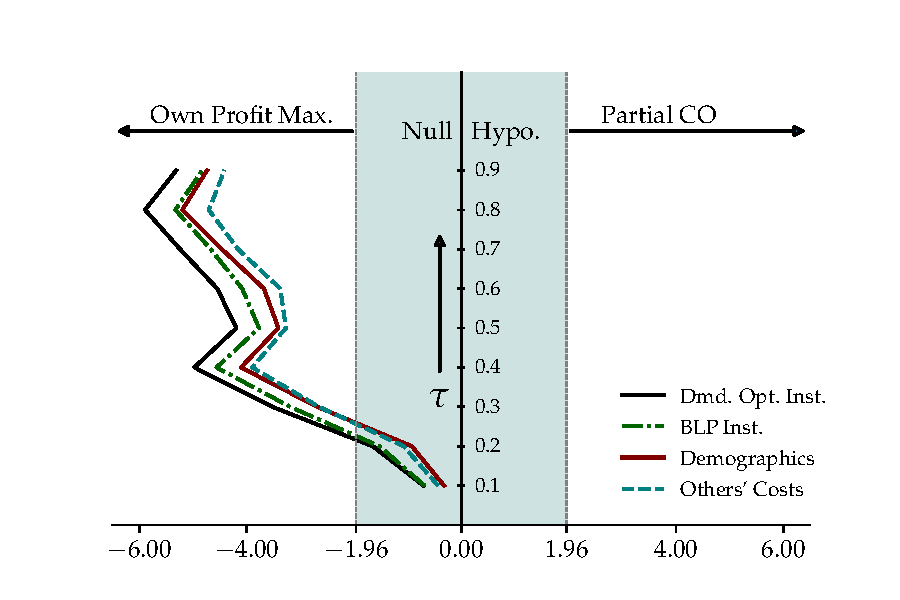
\includegraphics[height=\textheight]{resources/tau_figure2.pdf}
\end{center}
\end{frame}








\end{document}

